\subsubsection{Incremento 11}
\textit{\textbf{Periodo}: dal 2021-04-26 al 2021-04-29}

\myparagraph{Obiettivi}
Gli obiettivi definiti per questo incremento sono i seguenti:
\begin{itemize}
\item implementazione di feedback all'utente e visualizzazione errori;
\item implementazione requisiti obbligatori mancanti;
\item incremento della documentazione.
\end{itemize}

\myparagraph{Attività}
Per raggiungere gli obiettivi, vengono svolte le seguenti attività:
\begin{itemize}
\item \textbf{codifica}: 
\begin{itemize}
\item implementazione feedback all'utente;
\item implementazione della visualizzazione di errori;
\item implementazione requisiti obbligatori mancanti; 
\end{itemize} 

\item \textbf{ampliamento documentazione e verifiche}:
\begin{itemize}

\item incremento del \MUv{0.1.0} in base alle funzionalità aggiunte;
\item incremento del \MMv{0.1.0} in base alle funzionalità aggiunte;
\item incremento del \Glossariov{3.0.0};
\item rilevazione e registrazione di metriche, esiti di verifica e obiettivi di qualità;
\item aggiornamento dei rischi rilevati;
\item calcolo e registrazione del consuntivo di periodo.
\end{itemize}

\end{itemize}
\myparagraph{Diagramma di Gantt}
\begin{figure}[H]
\centering

\centerline{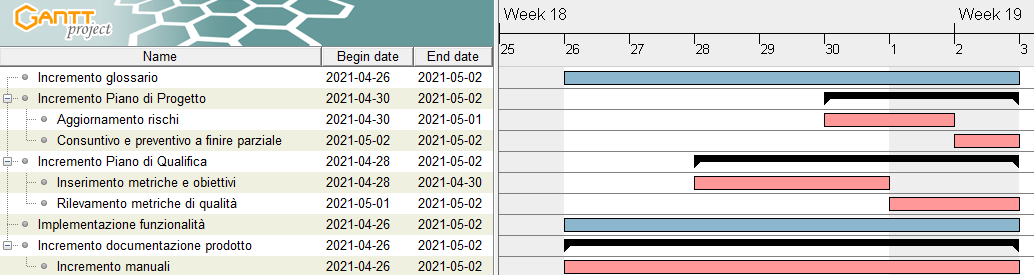
\includegraphics[scale=0.6]{res/Pianificazione/Fasi/VerificaIncrementi/ganttIncremento11}}
\caption{Diagramma di Gantt per l'incremento 11}
\end{figure}